% !TeX root = ../seminar.tex
\section{The Simulation}
\frame{\sectionpage}

\begin{frame}{A Monte Carlo of the bulge sky}
\centering
\vspace{1mm}
\begin{tikzpicture}[font=\footnotesize, execute at begin node={\hyphenpenalty=10000},
    inb/.style={terminator, fill=orange!12, text width=2.5cm, align=center, minimum height=1.25cm},
    row/.style={terminator, fill=blue!8, text width=13.6cm, align=center, minimum height=2.1em},
    resb/.style={terminator, fill=green!15, align=center, minimum height=2.3em}]
  \node[inb] (g) at (0,0)     {\textbf{Galaxy}\\ Besan\c{c}on model};
  \node[inb] (d) at (2.9,0)   {\textbf{Dust}\\ 3D maps};
  \node[inb] (p) at (5.8,0)   {\textbf{Lenses}\\ stars, BHs, NSs};
  \node[inb] (s) at (8.7,0)   {\textbf{Schedules}\\ LSST, GBTDS};
  \node[inb] (e) at (11.6,0)  {\textbf{Noise}\\ per visit};
  \uncover<2->{
  \node[row] (sky) at (5.8,-1.5) {$1{,}829$ sightlines over $68$\,deg$^2$};
  \foreach \n in {g,d,p,s,e} \path[connector] (\n.south) -- (\n.south |- sky.north);}
  \uncover<3->{
  \node[row] (mc) at (5.8,-2.55) {each sightline: draw $\to$ simulate both surveys $\to$ detect $\to$ forecast};
  \path[connector] (sky) -- (mc);}
  \uncover<4->{
  \node[row] (tab) at (5.8,-3.6) {event table: truth, who detects, forecast errors};
  \path[connector] (mc) -- (tab);}
  \uncover<5->{
  \node[resb, text width=5.6cm] (w) at (2.5,-4.85) {weight by event rate $\to$ the sky};
  \node[resb, text width=5.6cm] (an) at (9.1,-4.85) {analyses and yields};
  \path[connector] (tab.south -| w.north) -- (w.north);
  \path[connector] (w) -- (an);}
\end{tikzpicture}
\vfill
\refnote{Built on Dr.\ Sajadian's microlensing simulation (Magellanic Clouds), extended to two observatories.
\ads{2003A\%26A...409..523R}{Robin et al.\ 2003};
\ads{2019ApJ...887...93G}{Green et al.\ 2019};
\ads{2025ApJ...992...39Z}{Zucker et al.\ 2025};
\ads{1989ApJ...345..245C}{Cardelli et al.\ 1989}}
\note{\begin{itemize}
  \item Galaxy: Besan\c{c}on densities and a synthetic colour--magnitude diagram; magnitudes in $ugrizy$ and F146.
  \item Dust: $A_V(D)$ from Bayestar and DECaPS, converted with the CCM89 law.
  \item Lenses: ordinary stars and remnants, black holes, or neutron stars (one population per run).
  \item Schedules: Rubin's simulated LSST visit list; Roman's GBTDS seasons, fields and cadence.
  \item Sky: $0.1^\circ$ grid inside Roman's fields, $0.2^\circ$ outside; each sightline carries its area.
  \item The Monte Carlo does not draw events in proportion to the rate, so every event is weighted by its event rate.
\end{itemize}}
\end{frame}

\begin{frame}{Simulating one event}
\centering
\vspace{2mm}
\begin{tikzpicture}[font=\footnotesize, execute at begin node={\hyphenpenalty=10000},
    st/.style={terminator, fill=blue!8, text width=2.7cm, align=center, minimum height=3.2em},
    q/.style={terminator, fill=yellow!25, text width=2.7cm, align=center, minimum height=3.2em},
    nb/.style={draw=none, font=\scriptsize\itshape, text=jdgrey}]
  \node[st] (src) at (0,0)     {\textbf{Source}\\ star, distance, dust};
  \node[st] (len) at (3.75,0)  {\textbf{Lens}\\ mass, distance, velocity};
  \node[q]  (vis) at (7.5,0)   {\textbf{Visible?}};
  \node[st] (dat) at (11.25,0) {\textbf{Data}\\ at every real visit};
  \node[q]  (det) at (11.25,-2.2) {\textbf{Detected?}\\ $\Delta\chi^2\ge500$};
  \node[st] (fis) at (7.5,-2.2)   {\textbf{Fisher forecast}\\ three times};
  \node[st] (row) at (3.75,-2.2)  {\textbf{Event table}};
  \node[q]  (done) at (0,-2.2)    {\textbf{Enough events?}};
  \path[connector] (src) -- (len);
  \path[connector] (len) -- (vis);
  \path[connector] (vis) -- node[nb, above] {yes} (dat);
  \path[connector] (dat) -- (det);
  \path[connector] (det) -- node[nb, above] {yes} (fis);
  \path[connector] (fis) -- (row);
  \path[connector] (row) -- (done);
  \path[connector] (done) -- node[nb, left] {no} (src);
\end{tikzpicture}

\vspace{8mm}
\uncover<2->{Rubin from \textbf{Earth}, Roman from \textbf{L2}: two slightly different light curves}
\vfill
\refnote{Detection criterion as in \ads{2019ApJS..241....3P}{Penny et al.\ 2019, ApJS 241, 3}}
\note{\begin{itemize}
  \item Lens distance drawn in proportion to the event rate; $u_0\le3$; $t_0$ anywhere in the ten years.
  \item Visible: bright enough at the peak and not saturated, in two Rubin bands or in Roman's F146.
  \item Data: magnification and centroid shift with parallax at every real visit; each instrument's noise added.
  \item Detected: $\Delta\chi^2\ge500$ against a constant star and three consecutive points above $3\sigma$; tested on
        Rubin's data, Roman's and both. Every draw is kept, detected or not, for efficiencies.
  \item Labels: detected by Rubin only, Roman only, both, or only jointly.
\end{itemize}}
\end{frame}

\begin{frame}{Forecasting the measurement: three Fisher matrices}
\vspace{2mm}
\begin{columns}[c]
\begin{column}{.42\linewidth}
\centering
Curvature of $\chi^2$ at the truth:
\[
  F_{jk} = \sum_i \frac{1}{\sigma_i^2}\,\frac{\partial m_i}{\partial\theta_j}\,\frac{\partial m_i}{\partial\theta_k}
\]
\[
  C = F^{-1}
\]
\vspace{2mm}
\uncover<2->{\textbf{characterised:}\\ $\tE>2\sigma_{\tE}$ and $\piE>2\sigma_{\piE}$}
\end{column}
\begin{column}{.54\linewidth}
\centering
\begin{tikzpicture}[font=\footnotesize,
    d/.style={terminator, fill=orange!15, text width=1.9cm, align=center},
    f/.style={terminator, fill=blue!8, text width=2.5cm, align=center},
    s/.style={terminator, fill=green!15, text width=1.2cm, align=center}]
  \node[d] (rd) at (0,1.3)  {Rubin's data};
  \node[d] (od) at (0,-1.3) {Roman's data};
  \node[f] (fr) at (3.1,1.3)  {$F^{\rm Rubin}$};
  \node[f] (fo) at (3.1,-1.3) {$F^{\rm Roman}$};
  \node[f] (fj) at (3.1,0)    {$F^{\rm Rubin}+F^{\rm Roman}$};
  \node[s] (sr) at (5.9,1.3)  {$\sigma_{\rm Rubin}$};
  \node[s] (sj) at (5.9,0)    {$\sigma_{\rm joint}$};
  \node[s] (so) at (5.9,-1.3) {$\sigma_{\rm Roman}$};
  \path[connector] (rd) -- (fr); \path[connector] (od) -- (fo);
  \path[connector] (fr) -- (fj); \path[connector] (fo) -- (fj);
  \path[connector] (fr) -- (sr); \path[connector] (fj) -- (sj); \path[connector] (fo) -- (so);
\end{tikzpicture}

\vspace{5mm}
\uncover<3->{%
\begin{beamercolorbox}[rounded=true,sep=5pt,wd=.95\linewidth]{block body alerted}
\centering Same event, three forecasts:\\ \textbf{what each survey adds}
\end{beamercolorbox}}
\end{column}
\end{columns}
\vfill
\refnote{Characterisation criterion: \ads{2025ApJS..276...10A}{Abrams et al.\ 2025}; separate photometric and astrometric
matrices as in \ads{2023AJ....165...96S}{Sajadian \& Sahu 2023}}
\note{\begin{itemize}
  \item Too many events to fit each one; $F^{-1}$ is the Cram\'er--Rao bound for the real sampling and noise.
  \item Photometric matrix: $u_0$, $\tE$, $t_0$, $\piE$, the direction $\xi$, and a source magnitude and blending per
        telescope. Astrometric matrix: $\tetE$, the source proper motion (2), $\piE$.
  \item The three forecasts share the source, blending, $u_0$ and dust, so the per-event ratios
        $\sigma_{\rm joint}/\sigma_{\rm Roman}$, $\sigma_{\rm joint}/\sigma_{\rm Rubin}$ isolate what each survey adds.
        Built-in check: $\sigma_{\rm joint}\le\sigma_{\rm single}$.
\end{itemize}}
\end{frame}

\begin{frame}{One simulated black hole}
\vspace{1mm}
\begin{columns}[c]
\begin{column}{.64\linewidth}
\centering
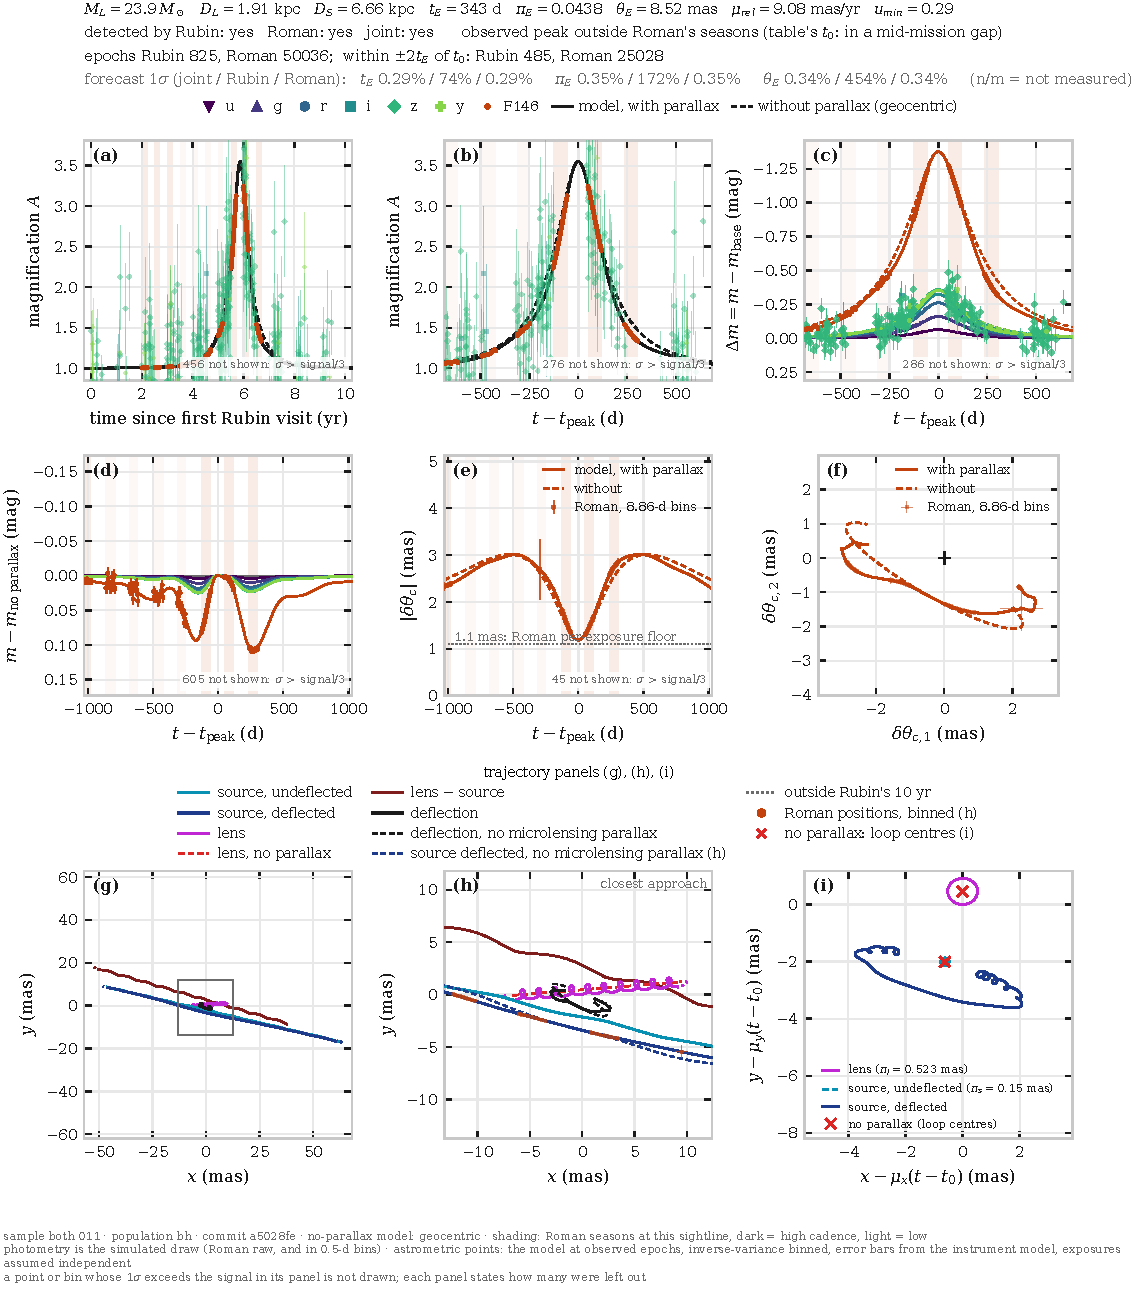
\includegraphics[width=.96\linewidth, trim=0 255 0 0, clip]{both_011_3x3}
\end{column}
\begin{column}{.32\linewidth}
\textbf{$23.9\,\Msun$ at $1.9$\,kpc}\\[3pt]
$\tE=343$\,d, $\tetE=8.5$\,mas
\vspace{6mm}

\uncover<2->{%
\begin{beamercolorbox}[rounded=true,sep=5pt,wd=\linewidth]{block body example}
Roman: \textbf{mass to $0.5\%$}\\[2pt]
Rubin alone: $\tE$ to $74\%$
\end{beamercolorbox}}
\end{column}
\end{columns}
\vfill
\refnote{This work, preliminary runs. Chosen for illustration, not typical.}
\note{\begin{itemize}
  \item Top row: photometry, Rubin's six bands and Roman's F146; Roman's seasons shaded (dark: high cadence).
  \item (d) the parallax signal; (e, f) the centroid shift (max.\ $3.0$\,mas) against Roman's $1.1$\,mas floor.
  \item Joint and Roman-alone precisions are the same here: $\tE$ to $0.3\%$, mass to $0.5\%$.
\end{itemize}}
\end{frame}
